\section{Ecosystem}
\begin{frame}
	\frametitle{The Julia Ecosystem}
  \begin{itemize}
    \item Packages and people
    \item http://juliacon.org/ in Berkeley in 2017
    \item https://discourse.julialang.org/
    \item https://juliaobserver.com/
    \item https://www.reddit.com/r/Julia/
    \item Repository gitters
    \item \#julia on Freenode
  \end{itemize}
\end{frame}

\begin{frame}[fragile]
	\frametitle{Package management}
  \begin{tiny}
  \begin{minted}{c}
julia> Pkg.status()
No packages installed.

julia> Pkg.add("Distributions")
INFO: Cloning cache of Distributions from git://github.com/JuliaStats/Distributions.jl.git
INFO: Cloning cache of NumericExtensions from git://github.com/lindahua/NumericExtensions.jl.git
INFO: Cloning cache of Stats from git://github.com/JuliaStats/Stats.jl.git
INFO: Installing Distributions v0.2.7
INFO: Installing NumericExtensions v0.2.17
INFO: Installing Stats v0.2.6
INFO: REQUIRE updated.

julia> Pkg.status()
Required packages:
 - Distributions                 0.2.7
Additional packages:
 - NumericExtensions             0.2.17
 - Stats                         0.2.6
  \end{minted}
  \end{tiny}
\end{frame}

\begin{frame}[fragile]
	\frametitle{Gadfly}
  \begin{tiny}
  \begin{minted}{julia}
using Gadfly
using RDatasets

plot(dataset("car", "SLID"), x="Wages", color="Language", Geom.histogram)
  \end{minted}
  \end{tiny}
  \begin{figure}[ht]
    \centering
    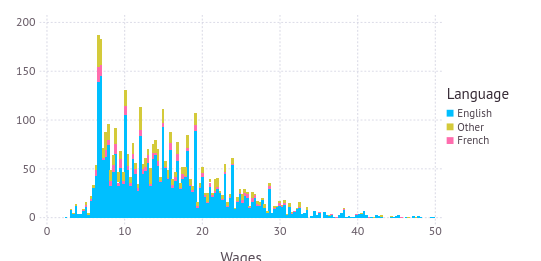
\includegraphics[width=0.6\textwidth]{gadfly0}
  \end{figure}
\end{frame}

\begin{frame}[fragile]
	\frametitle{Gadfly}
  \begin{tiny}
  \begin{minted}{julia}
using Gadfly
using RDatasets

iris = dataset("datasets", "iris")
p = plot(iris, x=:SepalLength, y=:SepalWidth, Geom.point);
img = SVG("iris_plot.svg", 6inch, 4inch)
draw(img, p)
  \end{minted}
  \end{tiny}
  \begin{figure}[ht]
    \centering
    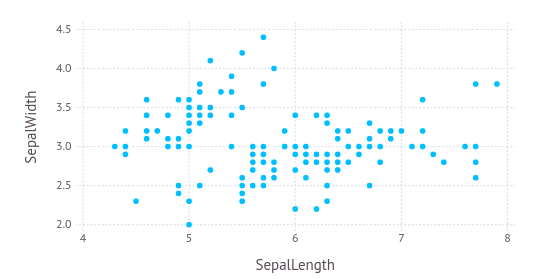
\includegraphics[width=0.6\textwidth]{gadfly1}
  \end{figure}
\end{frame}

\begin{frame}[fragile]
	\frametitle{Gadfly}
  \begin{tiny}
  \begin{minted}{julia}
fig1a = plot(iris, x="SepalLength", y="SepalWidth", Geom.point)
fig1b = plot(iris, x="SepalWidth", Geom.bar)
fig1 = hstack(fig1a, fig1b)
  \end{minted}
  \end{tiny}
  \begin{figure}[ht]
    \centering
    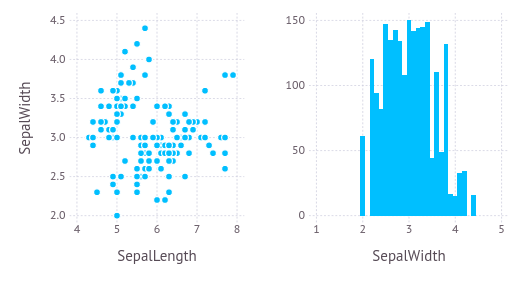
\includegraphics[width=0.6\textwidth]{gadfly2}
  \end{figure}
\end{frame}

\begin{frame}[fragile]
	\frametitle{Gadfly}
  \begin{tiny}
  \begin{minted}{julia}
using DataFrames

xs = 0:0.1:20

df_cos = DataFrame(x=xs,y=cos(xs),ymin=cos(xs) .- 0.5,ymax=cos(xs) .+ 0.5,f="cos")

df_sin = DataFrame(x=xs,y=sin(xs),ymin=sin(xs) .- 0.5,ymax=sin(xs) .+ 0.5,f="sin")

df = vcat(df_cos, df_sin)
p = plot(df, x=:x, y=:y, ymin=:ymin, ymax=:ymax, color=:f, Geom.line, Geom.ribbon)
  \end{minted}
  \end{tiny}
  \begin{figure}[ht]
    \centering
    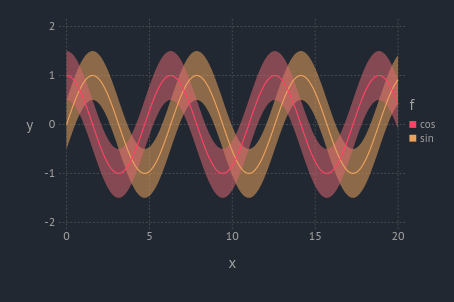
\includegraphics[width=0.5\textwidth]{gadfly3}
  \end{figure}
\end{frame}

\begin{frame}[fragile]
	\frametitle{Mocha}
  \begin{tiny}
  \begin{minted}{julia}
using Mocha

data  = HDF5DataLayer(name="train-data",source="train-data-list.txt",batch_size=64)
conv  = ConvolutionLayer(name="conv1",n_filter=20,kernel=(5,5),bottoms=[:data],tops=[:conv])
pool  = PoolingLayer(name="pool1",kernel=(2,2),stride=(2,2),bottoms=[:conv],tops=[:pool])
conv2 = ConvolutionLayer(name="conv2",n_filter=50,kernel=(5,5),bottoms=[:pool],tops=[:conv2])
pool2 = PoolingLayer(name="pool2",kernel=(2,2),stride=(2,2),bottoms=[:conv2],tops=[:pool2])
fc1   = InnerProductLayer(name="ip1",output_dim=500,neuron=Neurons.ReLU(),bottoms=[:pool2],
                          tops=[:ip1])
fc2   = InnerProductLayer(name="ip2",output_dim=10,bottoms=[:ip1],tops=[:ip2])
loss  = SoftmaxLossLayer(name="loss",bottoms=[:ip2,:label])

backend = DefaultBackend()
init(backend)

common_layers = [conv, pool, conv2, pool2, fc1, fc2]
net = Net("MNIST-train", backend, [data, common_layers..., loss])

exp_dir = "snapshots"
solver_method = SGD()
params = make_solver_parameters(solver_method, max_iter=10000, regu_coef=0.0005,
    mom_policy=MomPolicy.Fixed(0.9),
    lr_policy=LRPolicy.Inv(0.01, 0.0001, 0.75),
    load_from=exp_dir)
solver = Solver(solver_method, params)
  \end{minted}
  \end{tiny}
\end{frame}

\begin{frame}[fragile]
	\frametitle{Mocha}
  \begin{tiny}
  \begin{minted}{julia}
setup_coffee_lounge(solver, save_into="$exp_dir/statistics.jld", every_n_iter=1000)

# report training progress every 100 iterations
add_coffee_break(solver, TrainingSummary(), every_n_iter=100)

# save snapshots every 5000 iterations
add_coffee_break(solver, Snapshot(exp_dir), every_n_iter=5000)

# show performance on test data every 1000 iterations
data_test = HDF5DataLayer(name="test-data",source="test-data-list.txt",batch_size=100)
accuracy = AccuracyLayer(name="test-accuracy",bottoms=[:ip2, :label])
test_net = Net("MNIST-test", backend, [data_test, common_layers..., accuracy])
add_coffee_break(solver, ValidationPerformance(test_net), every_n_iter=1000)

solve(solver, net)

destroy(net)
destroy(test_net)
shutdown(backend)
  \end{minted}
  \end{tiny}
\end{frame}
